\documentclass[a4paper]{article}
\usepackage[english]{babel}
\usepackage[utf8]{inputenc}
\usepackage{graphicx}
\usepackage{enumitem}
\usepackage{blindtext}

\usepackage{multicol}

\graphicspath{ {./images/} }
\setlength\parindent{0pt}

\title{CS2200 Homework 6}
\author{Evan Wilcox}
\date{Due April 16, 2019}

\begin{document}
  \maketitle

  \begin{enumerate}
    %1
    \item
    \begin{enumerate}
      
      \item What are the variables of G? \\ R, S, T, X

      \item What are the terminals of G? \\ a, b

      \item Which is the start variable of G? \\ R

      \item  Give three strings in L(G). \\ ab \\ aab \\ babbaabb

      \item Give three strings not in L(G). \\ ba \\ baab \\ ababa

      \item True or False: T $\rightarrow$* aba. \\ True

      \item True or False: T $\rightarrow$* aba. \\ True

      \item True or False: T  $\rightarrow$* T. \\ False

      \item True or False: T $\rightarrow$* T . \\ False

      \item True or False: XXX  $\rightarrow$* aba. \\ True

      \item True or False: X  $\rightarrow$* aba. \\ False

      \item True or False: T $\rightarrow$* XX. \\ True

      \item True or False: T  $\rightarrow$* XXX. \\ True

      \item True or False: S $\rightarrow$* $\epsilon$. \\ False

      \item  Give a description in English of L(G). \\ 

    \end{enumerate}

    %2
    \item
    \begin{enumerate}
      
      \item \{w $|$ w contains at least three 1's\}
      \begin{enumerate}

        \item S $\rightarrow$ P1P1P1P

        \item A $\rightarrow$ A0$|$A1$|\epsilon$ \\

      \end{enumerate}

      \item \{w $|$ w starts and ends with the same symbol\}
      \begin{enumerate}

        \item S $\rightarrow$ 0A0$|$1A1$|0|1$

        \item A $\rightarrow$ 0A$|$1A$|\epsilon$ \\

      \end{enumerate}

      \item  \{w $|$ the length of w is odd\}
      \begin{enumerate}

        \item S $\rightarrow$ ASA$|$A

        \item A $\rightarrow$ $0|1$ \\

      \end{enumerate}

      \item \{w $|$ the length of w is odd and its middle symbol is a 0\}
      \begin{enumerate}

        \item S $\rightarrow$ ASA$|$0

        \item A $\rightarrow$ $0|1$ \\

      \end{enumerate}

      \item \{w $|$ w = wR, that is, w is a palindrome\}
      \begin{enumerate}

        \item S $\rightarrow$ 0S0$|$1S1$|$0$|$1$|\epsilon$ \\

      \end{enumerate}

      \item The empty set
      \begin{enumerate}

        \item S $\rightarrow$ S \\

      \end{enumerate}

    \end{enumerate}

    %3
    \item The structure of the .pda file should be as follows: \\
    One line beginning with an A followed by the characters in the pda's tape alphabet.
    One line beginning with a K followed by the characters in the pda's stack alphabet
    and the first character should be the end stack character. One line per state starting
    with a S followed by the name of the state and a boolean indicating if the state
    is a final state. One line starting with a B followed by the name of the starting
    state. One line per delta Starting with a D followed by the state you are in, the
    character you see on the tape, the character you see on the stack, the character 
    to replaced on the stack, and state you are going to. The @ should be used for the 
    empty string. One line per input to be tested starting with a T then the string, 
    immediately followed by a line starting with an O for the output. \\
    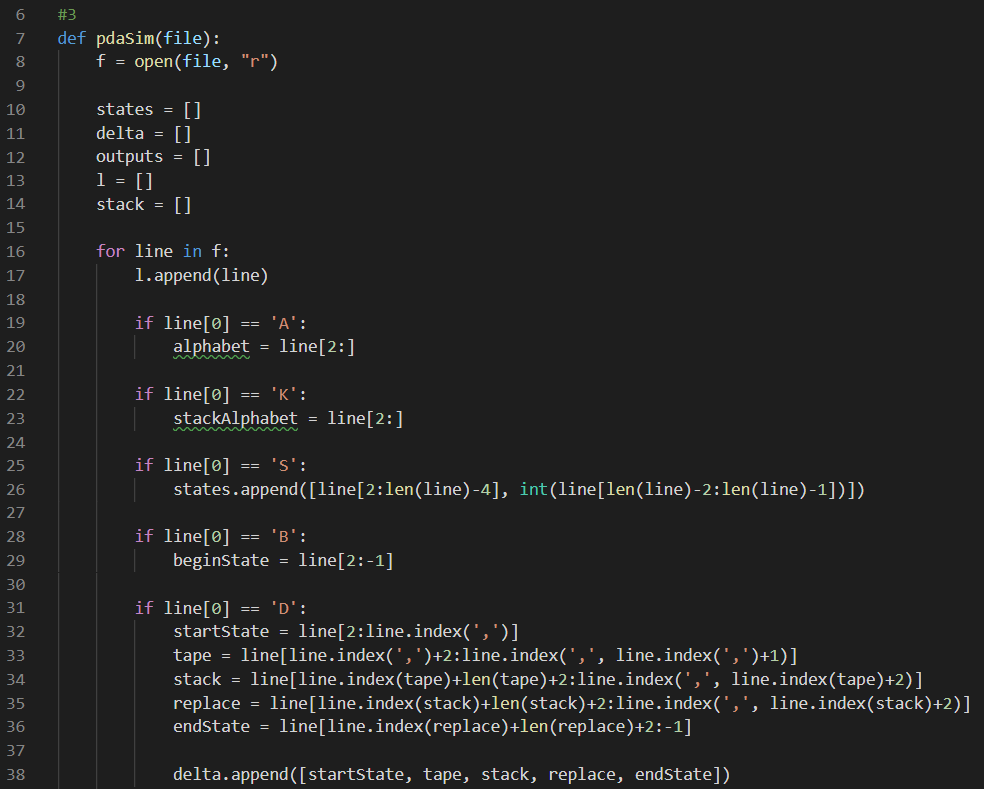
\includegraphics[scale=0.5]{3a} \\
    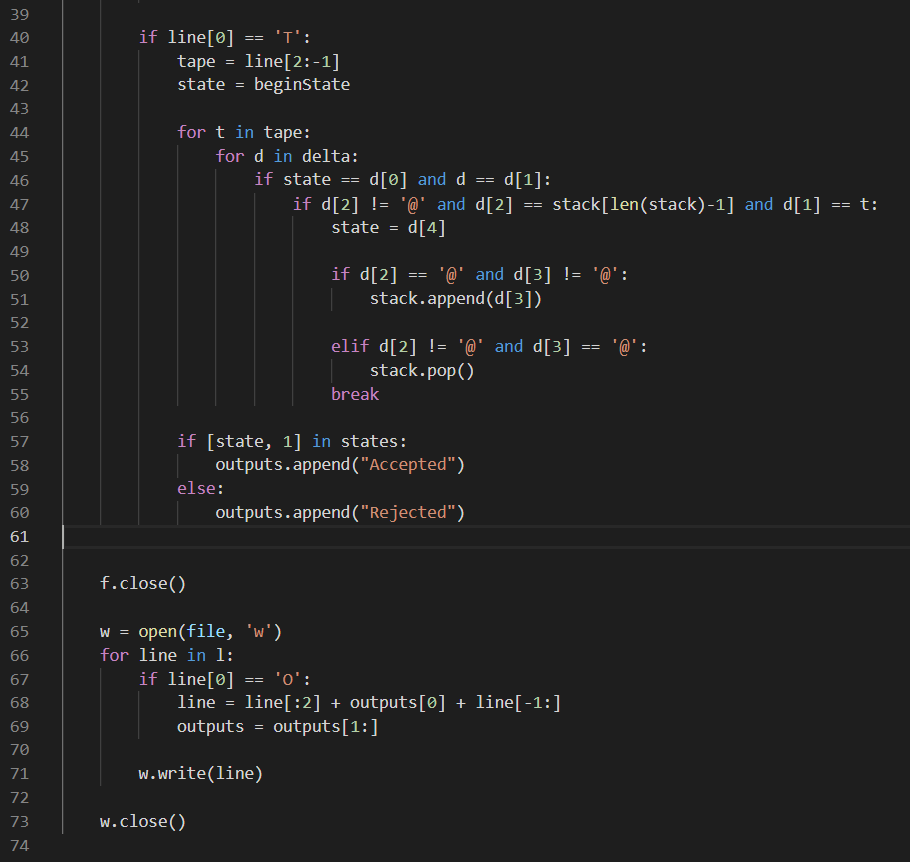
\includegraphics[scale=0.5]{3b} \\


    \newpage
    %5
    \item[5.]
    \begin{enumerate}
      
      \item 
      x \\
      \begin{tabular}{ |l|l|l| } \hline
        Rule & Application & Result \\ \hline
        Start $\rightarrow$ E & Start & E \\ \hline
        E $\rightarrow$ T & E & T \\ \hline
        T $\rightarrow$ F & T & F \\ \hline
        F $\rightarrow$ x & F & x \\ \hline
      \end{tabular}
      \vspace{1cm}
      
      x+x \\
      \begin{tabular}{ |l|l|l| } \hline
        Rule & Application & Result \\ \hline
        Start $\rightarrow$ E & Start & E \\ \hline
        E $\rightarrow$ E+T & E & E + T \\ \hline
        E $\rightarrow$ T & E + T & T + T \\ \hline
        T $\rightarrow$ F & T + T & F + T \\ \hline
        F $\rightarrow$ x & F + T & x + T \\ \hline
        T $\rightarrow$ F & x + T & x + F \\ \hline
        F $\rightarrow$ x & x + F & x + x \\ \hline
      \end{tabular}
      \vspace{1cm}

      (x$\times$x)+x \\
      \begin{tabular}{ |l|l|l| } \hline
        Rule & Application & Result \\ \hline
        Start $\rightarrow$ E & Start & E \\ \hline
        E $\rightarrow$ E + T & E & E + T \\ \hline
        E $\rightarrow$ T & E + T & T + T \\ \hline
        T $\rightarrow$ F & T + T & F + T \\ \hline
        F $\rightarrow$ (E) & F + T & (E) + T \\ \hline
        E $\rightarrow$ T & (E) + T & (T) + T \\ \hline
        E $\rightarrow$ E $\times$ T & (T) + T & (T$\times$F) + T \\ \hline
        T $\rightarrow$ F & (T$\times$F) + T & (F$\times$F) + T \\ \hline
        F $\rightarrow$ x & (F$\times$F) + T & (x$\times$F) + T \\ \hline
        F $\rightarrow$ x & (x$\times$F) + T & (x$\times$x) + T \\ \hline
        T $\rightarrow$ F & (x$\times$x) + T & (x$\times$x) + F \\ \hline
        F $\rightarrow$ x & (x$\times$x) + F & (x$\times$x) + x \\ \hline
      \end{tabular}
      \vspace{1cm}
      
      ((x)) \\
      \begin{tabular}{ |l|l|l| } \hline
        Rule & Application & Result \\ \hline
        Start $\rightarrow$ E & Start & E \\ \hline
        E $\rightarrow$ T & E & T \\ \hline
        T $\rightarrow$ F & T & F \\ \hline
        F $\rightarrow$ (E) & F & (E) \\ \hline
        E $\rightarrow$ T & (E) & (T) \\ \hline
        T $\rightarrow$ F & (T) & (F) \\ \hline
        F $\rightarrow$ (E) & (F) & ((E)) \\ \hline
        E $\rightarrow$ T & ((E)) & ((T)) \\ \hline
        T $\rightarrow$ F & ((T)) & ((F)) \\ \hline
        F $\rightarrow$ x & ((F)) & ((x)) \\ \hline
      \end{tabular}


    \end{enumerate}


  \end{enumerate}

\end{document}